\chapter{Heterogeneous CSS Implementation}
\label{chapter4}


\section{Overview}

\section{Experimental Setup}

\begin{figure}[ht!]
	\centering
	\includegraphics[width=\textwidth,keepaspectratio]{images/Gill/figs/setup.eps}
    \caption{Experimental Test-Bed For Cooperative Sensing in Heterogeneous Network. Sensors 1, 2 and 4 are RTL-SDR units, sensor 3 is USRP N210 and TX is another USRP N210 unit which is used as a signal source for this work.} 
\label{expsetup}      
\end{figure}

\subsection{Transmitter Setup for CSS Measurements}
\begin{figure}[ht!]
	\centering
	\includegraphics[width=\textwidth,keepaspectratio]{images/Gill/figs/transmitter.eps}
    \caption{GNU Radio Flowgraph For Transmitter Running on USRP N210.} 
\label{transmitter}      
\end{figure}

\subsection{Sensor Nodes Setup}

\begin{figure}[ht!]
	\centering
	\includegraphics[width=\textwidth,keepaspectratio]{images/Gill/figs/normalizedenergy.eps}
    \caption{GNURadio Flowgraph For USRP and RTL-SDR sensor nodes.} 
\label{receiver}      
\end{figure}

The central frequency is kept at 450 MHz and the operating parameters of each sensor node is provided in the table.
\begin{table}[!ht]
\caption{Operating Characteristics of Sensor Nodes}
\centering
\vspace{-5pt}
\begin{tabular}{|c | c | c | c | c|}
\hline
Nodes      & $F_s$     & Gain  & FFT Size &  Bin Size \\ \hline
RTL-SDR-1  & 1.1 Msps  & 10 dB & 512      & 2.148 KHz \\ \hline
RTL-SDR-2  & 1.8 Msps  & 10 dB & 512      & 3.515 KHz\\ \hline
RTL-SDR-3  & 2.4 Msps  & 10 dB & 512      & 4.687 KHz\\ \hline
USRP N210  & 7.2 Msps  & 10 dB & 512     &  14.062 KHz\\ 
\hline
\end{tabular}
\vspace{-5pt}
\label{table1}
\end{table}

\section{Hard Fusion}
\label{hardfusion}
The flowchart describes the three hard data fusion schemes.
\begin{figure}[ht!]
	\centering
	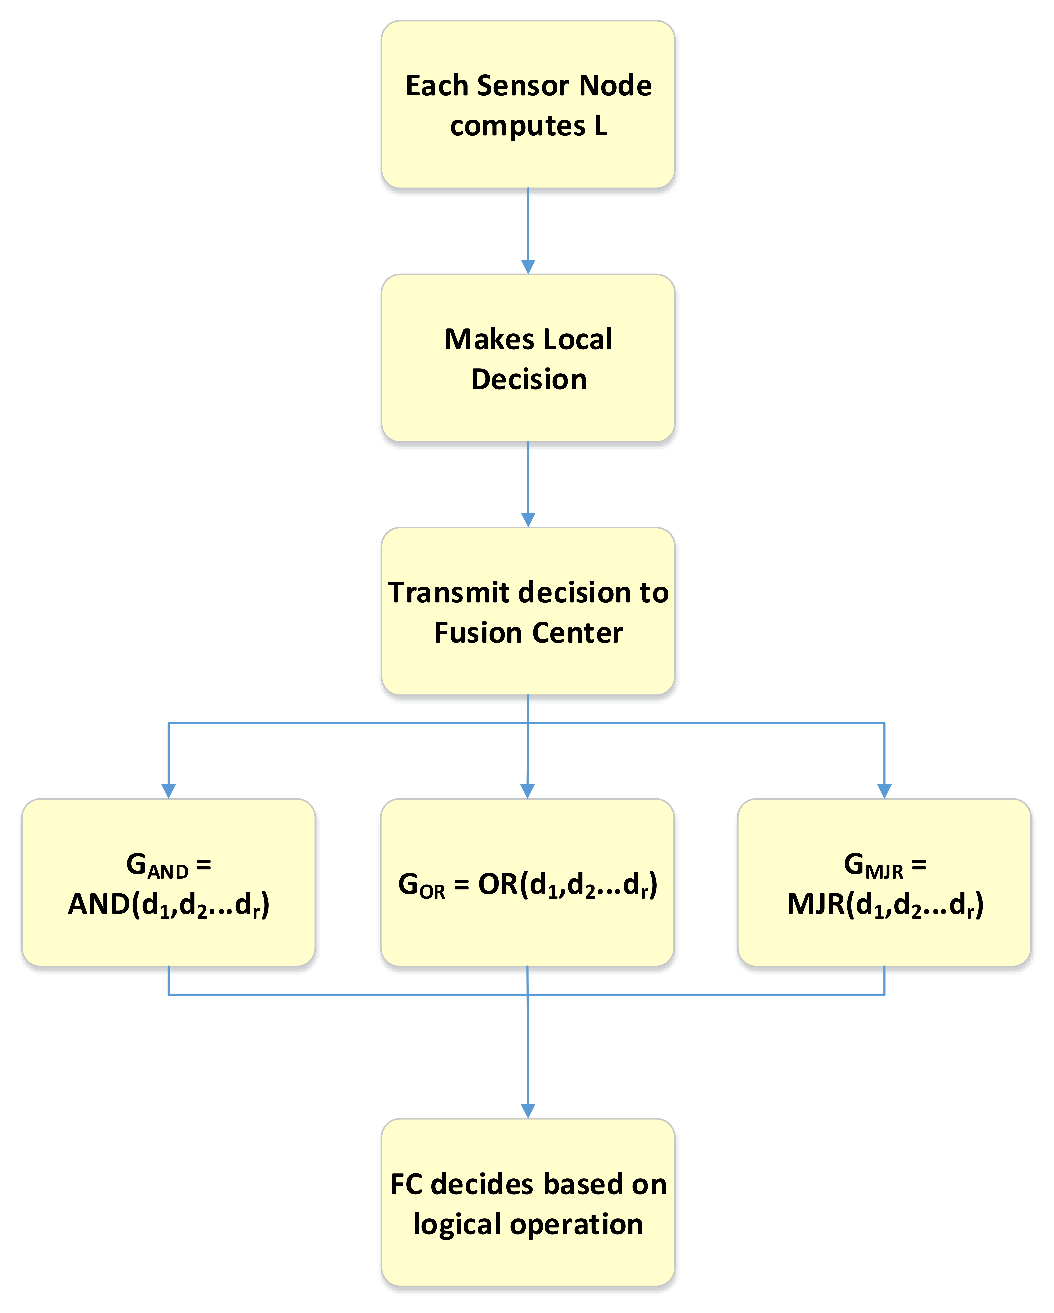
\includegraphics[width=\textwidth,height=10cm,keepaspectratio]{images/Gill/figs/hardfusion.eps}
\caption{Flowchart showing AND, OR and Majority Rule Fusion schemes..} 
\label{hard}      
\end{figure}


\section{Soft Fusion}

\subsection{Maximum Normalized Energy Scheme}

\begin{figure}[ht!]
	\centering
	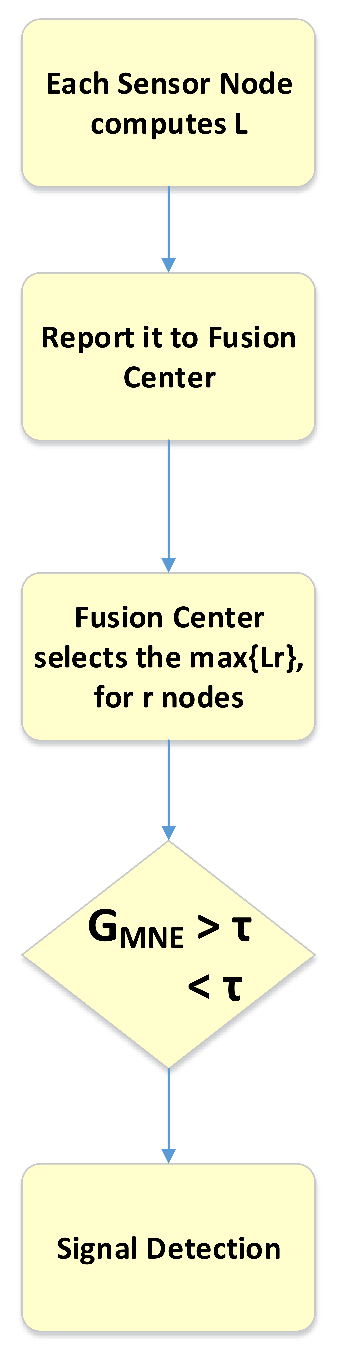
\includegraphics[width=\textwidth,height=10cm,keepaspectratio]{images/Gill/figs/mnescheme.eps}
\caption{Flowchart showing Equal Gain Combining Scheme.} 
\label{mnescheme}      
\end{figure}

\subsection{Equal Gain Combining Scheme}
\begin{figure}[ht!]
	\centering
	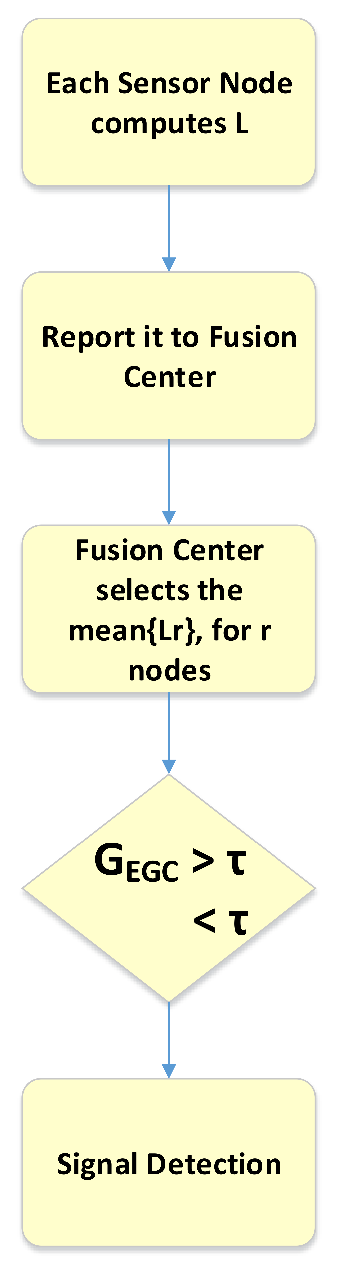
\includegraphics[width=\textwidth,height=10cm,keepaspectratio]{images/Gill/figs/egcscheme.eps}
\caption{Flowchart showing Maximum Normalized Energy Scheme.} 
\label{egcscheme}      
\end{figure}


\section{Summary}
This chapter outlined and examined the topics of jamming and anti-jamming techniques, and provided a foundation in communication system theory and advanced equalizer design.  Secondly it setup an understanding of Software-Defined Radio, the power of such an architecture, and examples of implementations and existing software for future designs.  Next, this thesis will consider a new anti-jamming technique and design an implementation of such a system.  After the implementation is investigated, the result of specific experiments on such an implementation will be analyzed.\\
